\documentclass[12pt,fleqn]{article}\usepackage{../../common}
\begin{document}
Say�sal Kontrol ve S�n�r De�er Problemleri (BVP)

Bu b�l�mde optimal kontrol problemlerini say�sal ��zmenin y�ntemlerini
g�rece�iz. 

Rayleigh Problemi

Bir elektrik devresi d���nelim, bu devre d�z voltaj� sal�n�ma �evirebiliyor, 

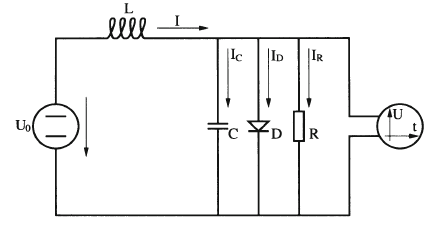
\includegraphics[width=20em]{phy_num_01.png}

Devreyi sol taraftan verilen $U_0(t)$ ile kontrol etmek m�mk�n [1,
sf. 189], [2, sf. 413]. Devreninin denklemi

$$
\ddot{x} = -x(t) + \dot{x}(t) ( 2.0 - p \dot{x}(t)^2 ) +  u(t)
$$

ki biz $p = 0.1$ se�ece�iz. ODE sistemi ��kartmak i�in $x_1 = x$, $x_2
= \dot{x}$ dersek,

$$
\dot{x_2} = -x_1 + (2.0 - 0.1 x_2^2)x_2 + 4 u(t)
$$

Acaba $x_1(t=0)=-5$ ve $x_2(t=0)=-5$ ba�lang�� �artlar� i�in,
$t_f=2.5$ an�na kadar kontrol� ve sal�n�m� az seviyede tutmaya
�al��sak nas�l bir kontrol uygulamam�z gerekir? 







[devam edecek]

Kaynaklar

[1] Bittner, {\em Variational calculus, optimal control and applications}

[2] Wilson, {\em Advanced Control using MATLAB}

\end{document}
